

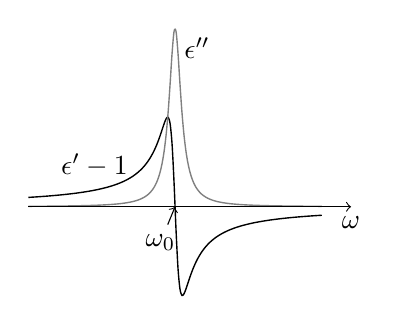
\begin{tikzpicture}[
declare function={ 
 w0 = 100;
 gamma = 1;
 amp = 2;
 epsr(\w) =  amp * (w0 ^2 - \w^2)/ ( (w0 ^2 - \w^2)^2 + gamma^2 * \w^2);
 epsi(\w) =  amp * gamma * \w / ( (w0 ^2 - \w^2)^2 + gamma^2 * \w^2);
  },
]
%\useasboundingbox (0,0) rectangle (5,5);
%\draw (0,0) rectangle (5,5);

\begin{axis}[no markers,
 samples=150, smooth,
     %     ymin=-0.3, ymax=1,
        axis y line=none,
          axis x line=none,
           width= 6.5cm]
           
\addplot [domain=90:110,  line width=0.5pt]    { epsr(x)};
\addplot [domain=90:110,  line width=0.5pt, gray]    { epsi(x)};

\addplot[->] coordinates   {(90,0) (112, 0)};
\node (s) [anchor= north] at (axis cs: 112,0) {$\omega$} ;
\node (w0) [anchor= north ] at (axis cs: 99,-0.002) {$\omega_0$} ;
\draw[->] (w0) -- (axis cs: 100,0);


\node [anchor= north] at (axis cs: 94.5,0.007) {$\epsilon' -1 $} ;
\node [anchor= north] at (axis cs: 101.5,0.02) {$\epsilon'' $} ;


           
\end{axis}

\end{tikzpicture}

